\section{Background}
The alpha parameter ($\alpha$) is a topographic diffusion coefficient, and influences both cross-slope sediment flux and bank erodibility.
While detailed investigation into a similar parameter in the Delft3D morphodynamic model has been conducted \citep{Baar2019}, a similar analysis has not been conducted using DeltaRCM or pyDeltaRCM.
The reduced complexity approach in the DeltaRCM model is inspired by the Bagnold-Ikeda formulation in \citet{Garcia2008}, \citep{Liang2015a}.

\section{Model Runs}
To test the influence of the $\alpha$ YAML parameter, runs with the following parameters were conducted in triplicate with alpha values of $\alpha = 0.01, 0.05, 0.1, 0.5, 1.0, 5.0, 10.0$.
The YAML below provides information about the parameter set used.\\

\noindent \texttt{YAML} configuration file: \vspace{-6pt}
\begin{boxedverbatim}
Length: 7500
Width: 15000
timesteps: 5000
L0_meters: 150.0
N0_meters: 250.0
dx: 50.0
h0: 5.0
Np_water: 2000
Np_sed: 2000
save_dt: 250000
\end{boxedverbatim}

\section{Results}
The influence of the alpha parameter can be seen when looking at the final topographies generated by the various models (Figure \ref{fig:alpha_topos}).
The effect diffusion of the topography has on the channels can be seen more clearly in Figure \ref{fig:alpha_transect} which provides a visualization of an azimuthal transect sliced through the system.
Finally, the width-to-depth ratios of the surface channels are also impacted by the different degrees of topographic diffusion (Figure \ref{fig:alpha_wd}).

\begin{sidewaysfigure}[!ht]
	\makebox[\textwidth][c]{
	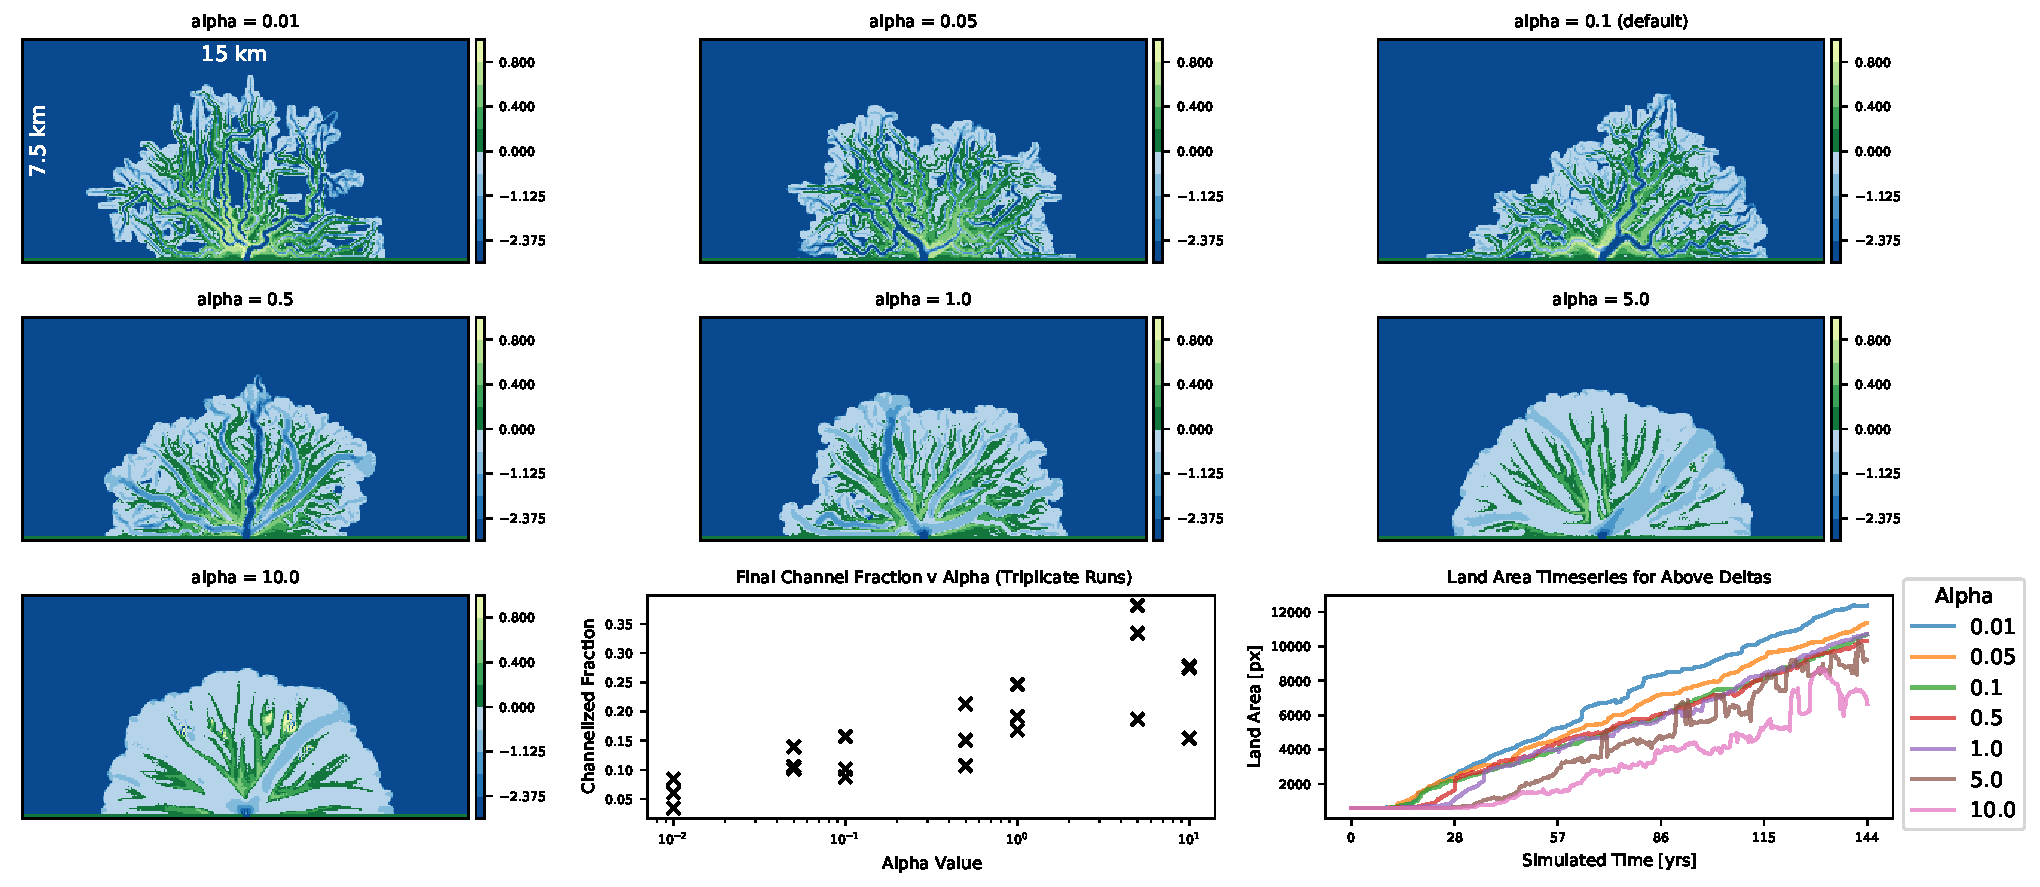
\includegraphics[width=\textwidth]{AlphaImpact/figs/alpha_results.pdf}
	}	
	\caption{Examples of the final topographies obtained for different values. \textit{Bottom, center:} Channelized fractions at the end of each model run as a function of the alpha parameter. \textit{Bottom, right:} Land area timeseries for one model per alpha parameter.}
	\label{fig:alpha_topos}
\end{sidewaysfigure}

\begin{sidewaysfigure}[!ht]
	\makebox[\textwidth][c]{
	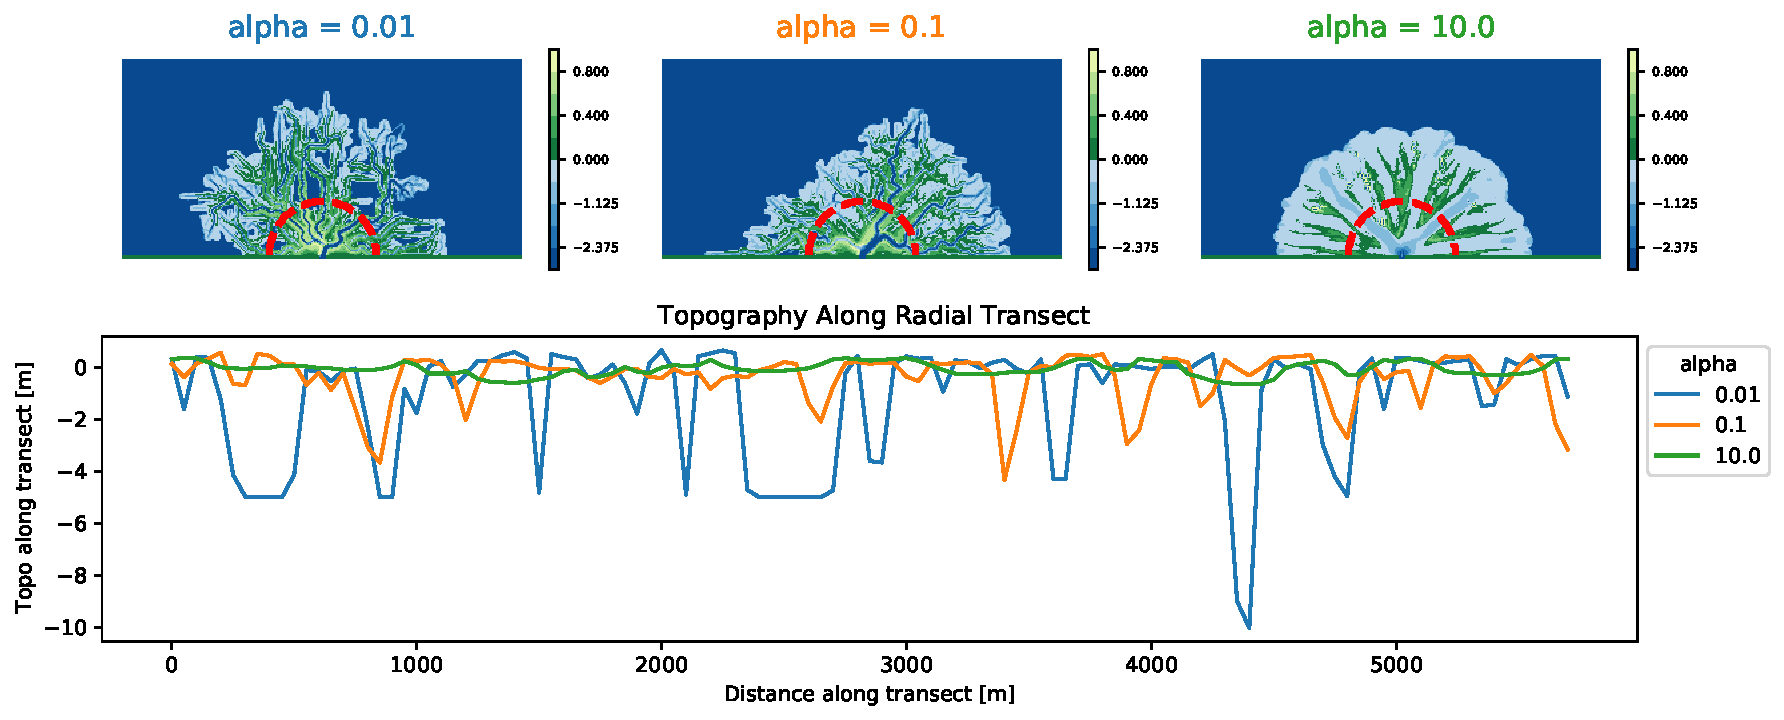
\includegraphics[width=\textwidth]{AlphaImpact/figs/topotransect_alpha.pdf}
	}	
	\caption{Topography transects for the lowest, default, and highest alpha values tested to visualize the impact of topographic diffusion on the channel geometries.}
	\label{fig:alpha_transect}
\end{sidewaysfigure}

\begin{figure}[!ht]
	\makebox[\textwidth][c]{
	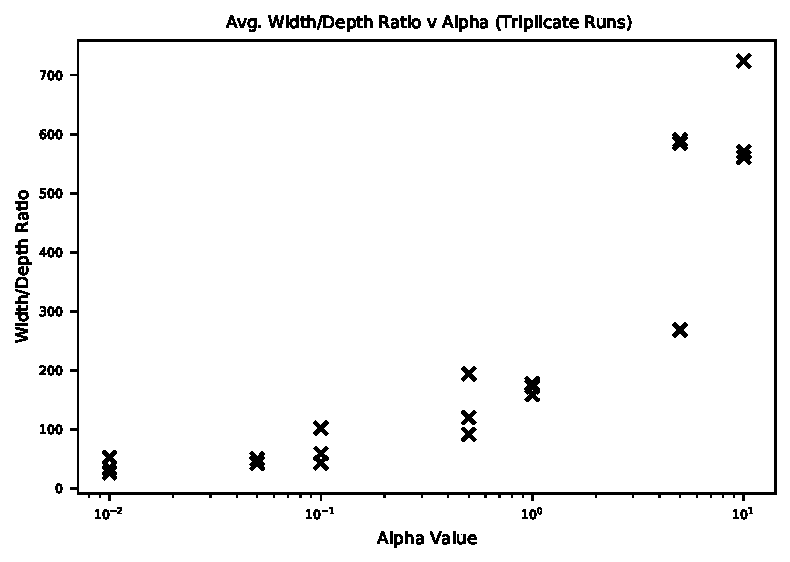
\includegraphics[width=\textwidth]{AlphaImpact/figs/widthdepth_alpha.pdf}
	}	
	\caption{Plot of average width-to-depth ratios as a function of the different alpha values. Width-to-depth ratios are calculated along the azimuthal transects visualized in Figure \ref{fig:alpha_transect}.}
	\label{fig:alpha_wd}
\end{figure}

\section{Conclusions}
The alpha parameter clearly influences the simulated deltas.
Values close to the default value of 0.1 appear to have only slight impacts on the topography and channel properties.
Once the alpha parameter deviates more significantly from its default, significant impacts to the visual appearance of the deltas as well as properties related to the channels occur.
These results appear consistent with those observed in \citet{Baar2019} when a similar property was tested using in Delft3D.

\clearpage
\bibliographystyle{plainnat}
\bibliography{bib/bib}